\section{Le contrôleur}

\subsection{le serveur tcp}

\indent Parmi les différentes parties du controleur, on trouve ce que nous avons baptisé le serveur tcp.
Ce dernier prend en charge les communications entre le programme qui gère l'aquarium et le client.\\
\indent Lors d'une requête du client, le serveur tcp va vérifier la validité de la requête et appeler les fonctions correspondantes.
Dans le cas d'un \textit{getFishescontinously},
il crée un thread actif en parallèle de son thread principal qui appelle tout le temps la fonction \textit{getFishes}.

\begin{figure}[!h]
\caption{\label{handlers} Diagramme de séquences}
\begin{center}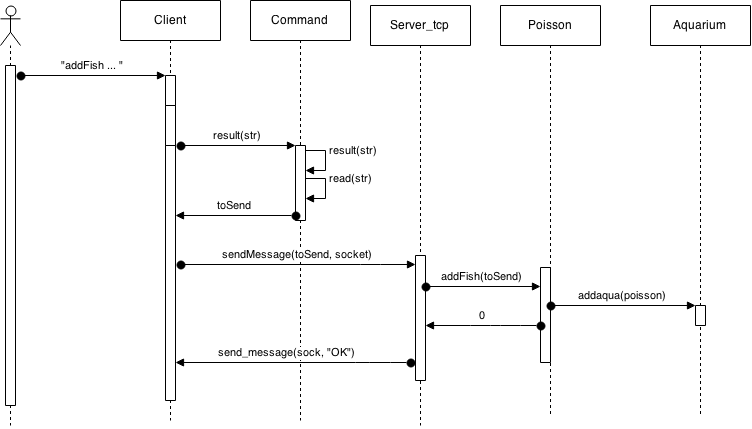
\includegraphics[scale=0.5]{Diagram}\end{center}
\end{figure}

D'autre part, le fonctionnement de cette partie est basée sur une simple aborescence de threads parmis lesquels nous
trouvons celui qui attend des requêtes à executer, et celui qui envoie les informations afin de rafraichir
l'aquarium du coté du client. Chacun des threads qui gère les requetes  est créé lors de l'acceptation
d'un client et est propre au client qui à pour identifiant le numéro de la socket qu'il utilise avec le serveur.

\begin{figure}[!h]
\caption{\label{handlers} Structure des clients côté serveur}
\begin{center}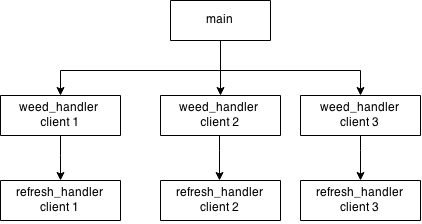
\includegraphics[scale=0.8]{thread}\end{center}
\end{figure}


Ainsi, lors d'une demande de deconnexion, le client demande à se déconnecter à l'aide de la requête \textit{exit},
le serveur reçoit le message et envoie la confirmation de déconnexion, fait un join de tous les threads et kill
et aussi éventuellement celui qui permet le rafraichissement, et fini par fermer la socket.
Néanmoins, meme si le client est déconnecté le serveur reste actif et attend d'autres clients potentiel,
via une boucle while munie d'une fonction accept propre au protocole tcp.
